%%%%%%%%%%%%%%%%%%%%%%%%%%%%%%%%%%%%%%%%%%%%%%%%%%%%%%%%%%%%%%%%%%%%%%%%%%%%%%%%
%neutrino_physics.tex: Chapter on neutrino physics:
%%%%%%%%%%%%%%%%%%%%%%%%%%%%%%%%%%%%%%%%%%%%%%%%%%%%%%%%%%%%%%%%%%%%%%%%%%%%%%%%
\chapter{Problem Setup and Overview }
\label{chapter:preliminaries}
%%%%%%%%%%%%%%%%%%%%%%%%%%%%%%%%%%%%%%%%%%%%%%%%%%%%%%%%%%%%%%%%%%%%%%%%%%%%%%%%

%%%%%%%%%%%%%%%%%%%%%%%%%%%%%%%%%%%%%%%%%%%%%%%%%%%%%%%%%%%%%%%%%%%%%%%%%%%%%%%%
In this chapter, we formalize our problem definition and present a brief overview of our system. We start with the problem definition : `` Given two captured image series of the same portion of a tree row from a monocular camera (i.e. cell phone, Go-Pro etc)- one from the front side of the row and one from the back side- we want to estimate the total fruit counts and locations for the captured portion of the row.'' See Figure~\ref{fig:concept} for an overview of the proposed system.
\begin{figure*}[ht!]
	\centering
	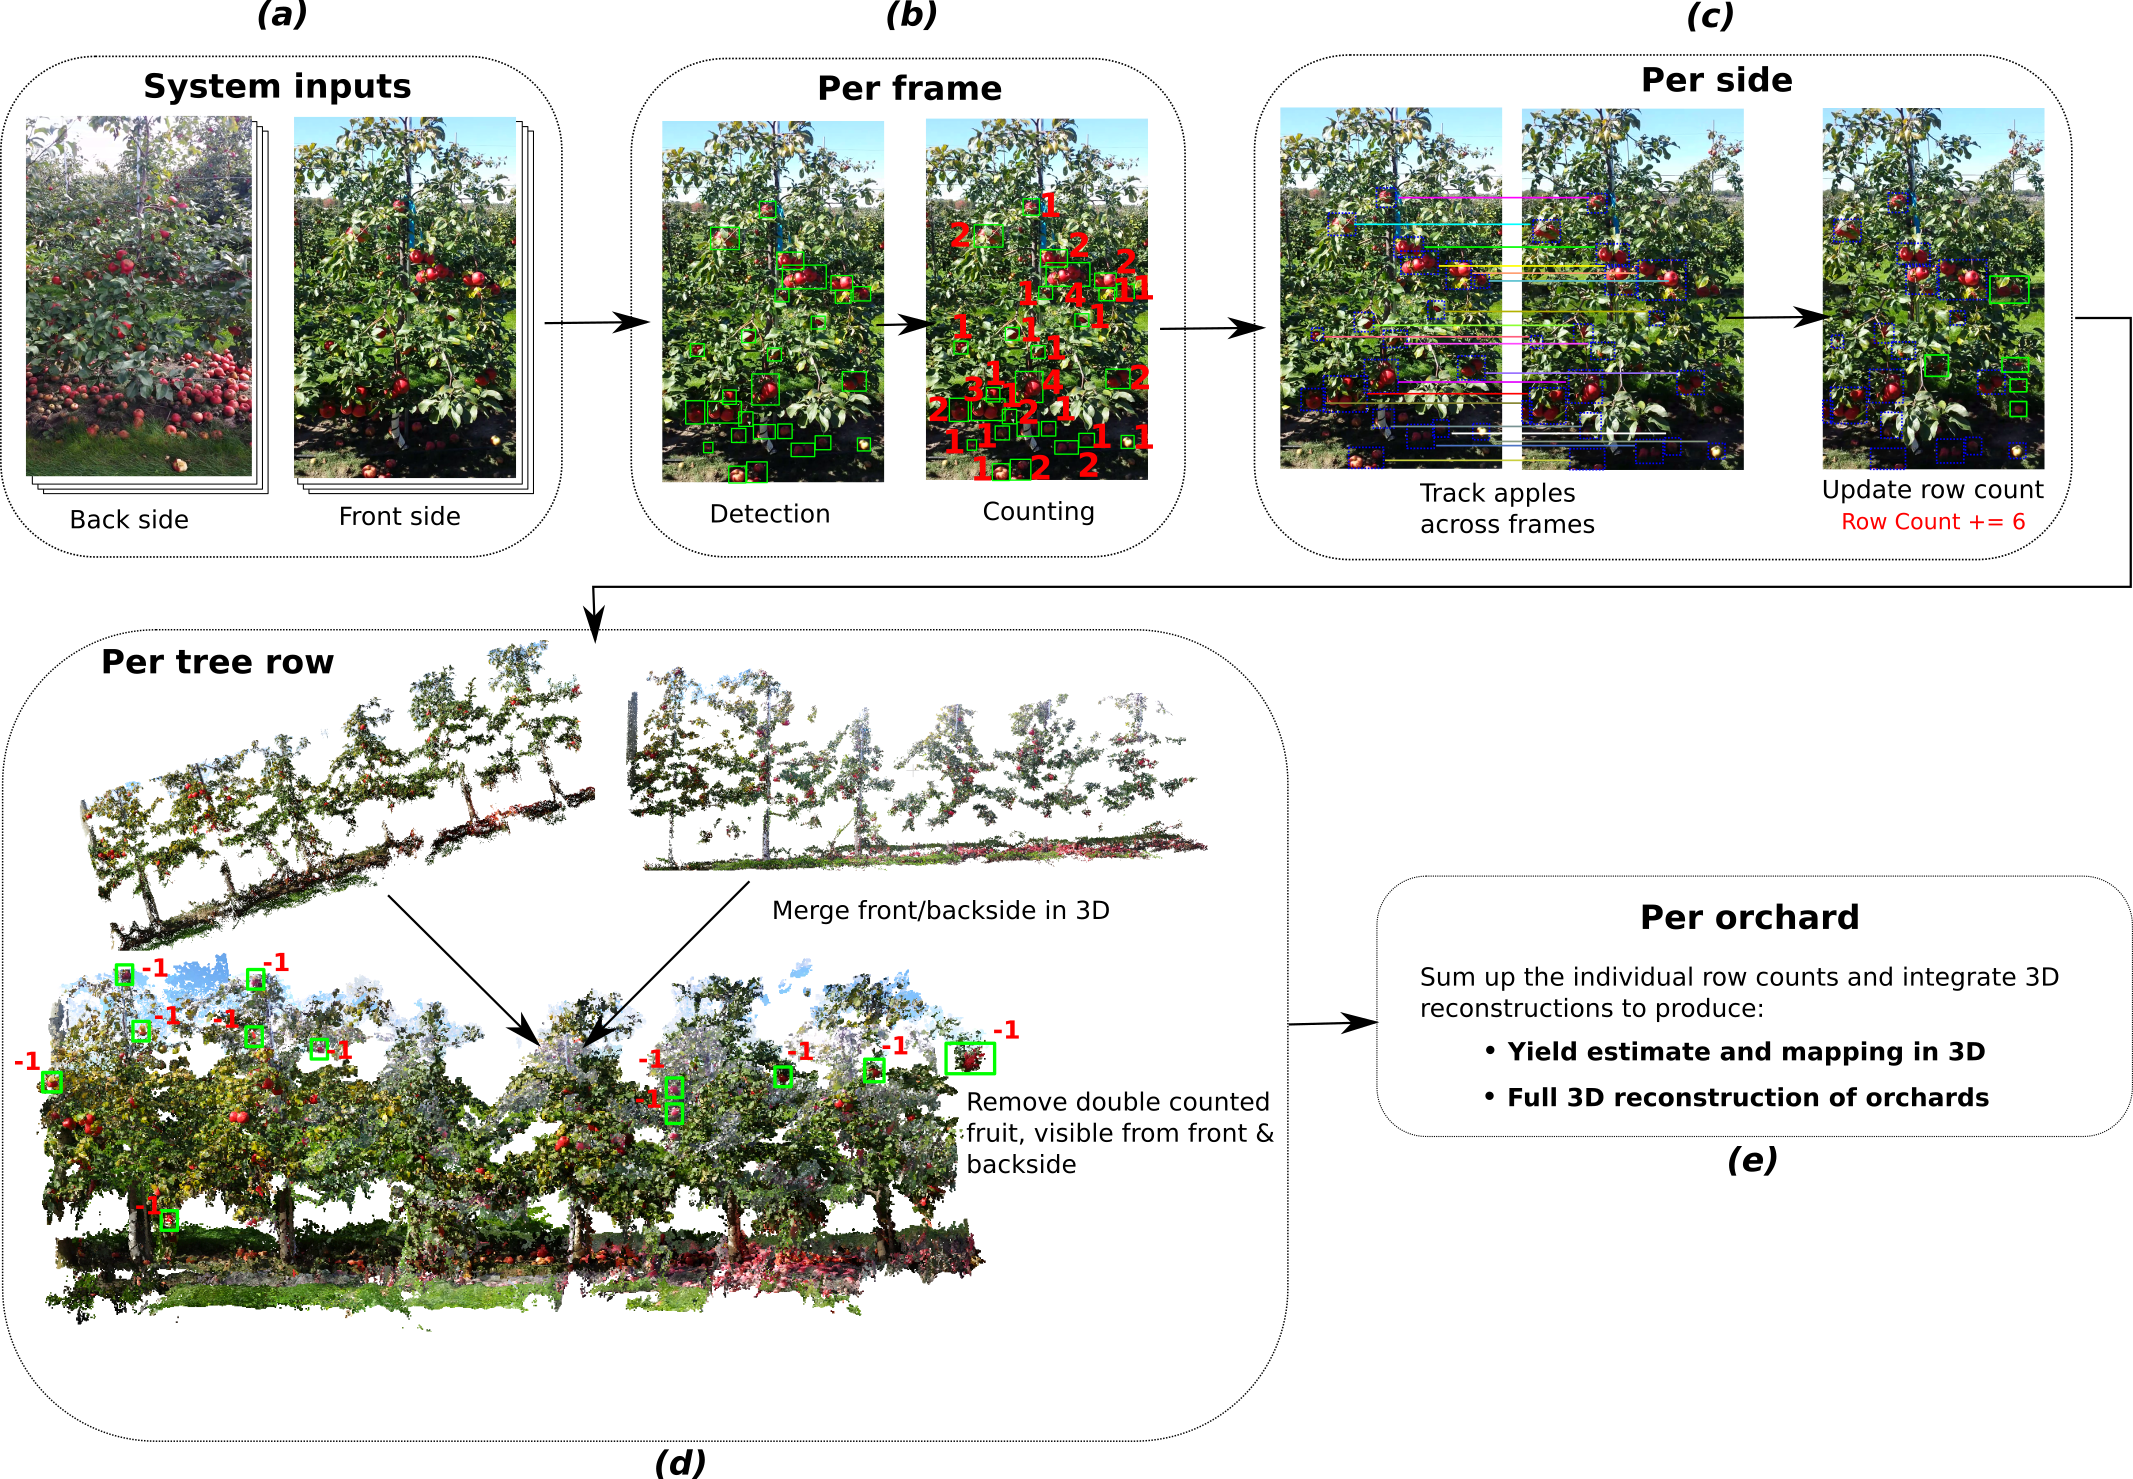
\includegraphics[width=\textwidth]{figures/prelim/conceptFigure.png}
	\caption{Overview of the yield estimation process. (a) Given two image sequences from the same portion of an orchard row, one from the front and one from the back. (b) Fruits are detected and counted in each frame. (c) Fruits are tracked across the image sequence to avoid double counting. As outputs, we have an image sequence per side, together with fruit locations and counts. (e) We reconstruct each image sequence in 3D and merge the two reconstructions into a single 3D model of the tree row. For yield estimation, we can now remove fruits visible from both sides of the tree row. (f) The pipeline produces yield estimates together with a 3D reconstruction and fruit mapping.}
	\label{fig:concept}
\end{figure*}
%
An end to end solution to this problem involves solving multiple sub-problems such as fruit detection, counting, tracking fruits across multiple views and merging fruit counts from both sides of a row. The presented system in this proposal strives to minimize the coupling between the solutions to different sub-problems. Essentially, the design goal is to ensure that the solution to a particular sub-problem can be changed without affecting others (i.e the fruit detection methods can be changed without affecting the counting methods). 

To ensure this logical separation, we divide our system into multiple components including: fruit detection, fruit counting, recovering scene geometry for tracking fruits from a single side, merging scene geometry from both sides of a row, and finally an accumulator for computing the actual yield.

Basically, the proposed system detects and counts fruits in individual images, and the fruits are tracked across an image sequence using estimated camera motion and scene geometry. Afterward, independent single side reconstructions are merged into a coherent 3D model. With the help of this model, the system eliminates duplicate fruit counts owing to fruits visible from both sides. Next, we provide a brief overview of all of these components.

%
\section{Fruit Detection}\label{subsec:syssegmentation}

The fruit detection module takes as input a color image for each frame, and outputs a binary mask which marks whether each pixel in the image belongs to the class \texttt{apple} (Fig.~\ref{fig:seg_pipeline}). In this proposal, we present two different approaches for fruit detection. 

Our first approach is a semi-supervised color-based clustering technique utilizing Gaussian Mixture Models (GMM) and Expectation Maximization (EM)~\cite{moon_expectation-maximization_1996} \cite{roy_vision-based_2018}. In this approach, the image is over-segmented into SLIC superpixels (\cite{achanta2012slic}), using the LAB~\cite{connolly1997study} colorspace. A single representative color (mean LAB color of the pixels within the superpixel) is assigned to each superpixel. Then superpixels are clustered by color into approximately $25$ color classes. Finally, it is determined for each class whether it describes apples, based on KL divergence (\cite{goldbergerKLdivergence}) from hand-labeled classes. These hand-labeled classes can be obtained from the unsupervised clusters of the first few frames of a particular video, to easily account for current lighting conditions and the color of the particular apple variety at its particular ripeness.

While the semi-supervised color-based clustering technique is intuitive and simple to train, it is hard to generalize across different datasets. To resolve this problem, we present a novel approach~\cite{hani_jfr_counting} based on a deep pixel-wise segmentation network, U-Net~\cite{ronneberger_u-net:_2015}. In this approach, each pixel in the image is assigned a class (apple/background), and our objective is to minimize the total classification error. We analyze the performances of both these approaches on multiple datasets. This component is presented in detail at Chapter~\ref{chapter:detection}




\section{Fruit Counting}\label{subsec:sysperframecounting}

\begin{figure}[!hbpt]
{\centering
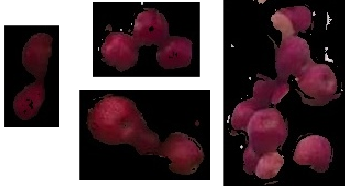
\includegraphics[height=2cm]{figures/prelim/capple1.png}
%\vspace{10mm} 
\vrule 
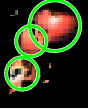
\includegraphics[height=2cm]{figures/prelim/gmmcomp.png}
%\vspace{10mm} 


\caption{
From left to right: Segmented images exhibiting complex geometry. Sample output of our algorithm on an individual cluster. \label{fig:counting_ex}}
}
\end{figure}

\begin{figure}[!hbpt]
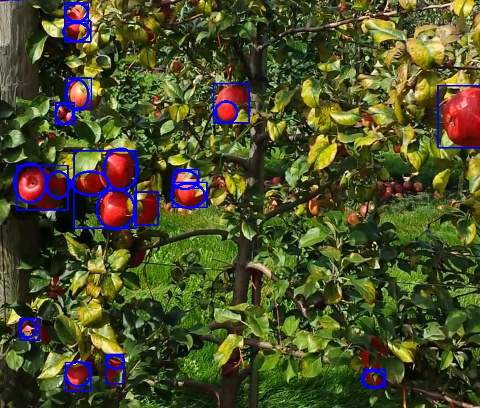
\includegraphics[width=.58\columnwidth]{figures/prelim/complex_count1.jpg}
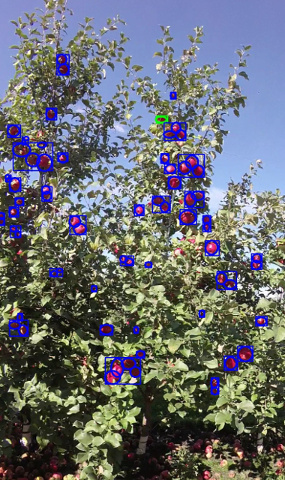
\includegraphics[width=.32\columnwidth]{figures/prelim/CountFullComplex11.jpg}
%%%
\caption{Sample output of our algorithm after the counting step. These two images show the difference in the number of pixels occupied by individual apples. Our algorithm works for both cases regardless of any tuning, whereas techniques such as Circular Hough Transform (CHT) need to be tuned for maximum/minimum fruit size for each individual case.}
\label{fig:full_count}
\end{figure}
The counting component takes as input the binary segmented mask for each frame, and outputs a set of bounding boxes and associated integers for each frame where each bounding box represents a connected cluster of fruits, and the integer is the estimated number of fruits in that cluster (Fig.~\ref{fig:counting_ex}, \ref{fig:full_count}).

First, a connected component analysis is performed on the binary fruit mask. Each connected component is examined separately, to determine how many fruits it contains. To estimate the fruit counts accurately, we developed a method based on a classic clustering technique: Gaussian Mixture Models (GMM) (\cite{em}). Our method provides both the counts and location of individual fruits in an input image. Our method models each fruit with a Gaussian probability distribution function (pdf) and each fruit cluster with a mixture of Gaussians. Afterward, we use a novel heuristic to find the correct number of components (i.e the number of fruits) in the mixture model. Additionally, we compared this approach to one of our latter work presented in \cite{hani_apple_2018}, which poses fruit counting as a multi-class classification problem. This module is presented in detail at Chapter~\ref{chapter:fruit_counting}. 

\section{Estimating Scene Geometry and Camera Motion}\label{subsec:syscammotion}

Tracking is an essential task to avoid double counting of fruits. For the purpose of yield mapping we need to track the fruits in the images captured from a single side of a tree row. Additionally, we also need to to track them from the other side of the row owing to fruits visible from both sides. We developed two separate components for this task. First, we designed a method that takes the entire sequence of images from a single side of a tree row, the detected fruit clusters and their counts as input. The output is a total count of unique apples seen in the frame sequence (Fig.~\ref{fig:tracking}, \ref{fig:mergecount}).

This component builds a dense reconstruction of the scene from a single side using incremental Structure from Motion. We developed a novel SfM pipeline where fruit contours are directly used for generating dense point matches. These matches are then used for computing the 3D scene structure and estimating camera motion. This component is presented in detail at Chapter~\ref{chapter:sfm}. Next, we present the component responsible for merging the scene geometry from both sides.

\begin{figure}[!hbpt]
{\centering
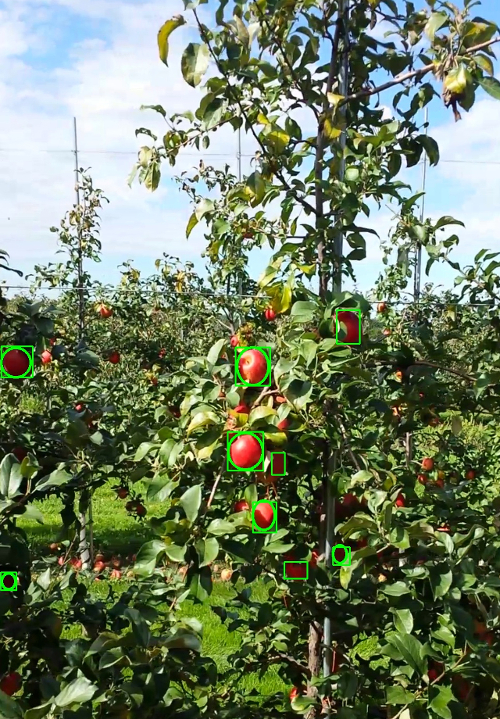
\includegraphics[width=0.3\columnwidth]{figures/prelim/tracking11.jpg}
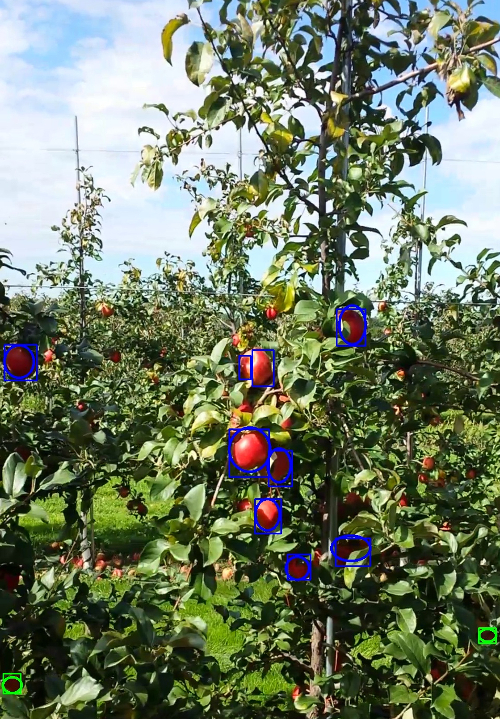
\includegraphics[width=0.3\columnwidth]{figures/prelim/tracking22.jpg}
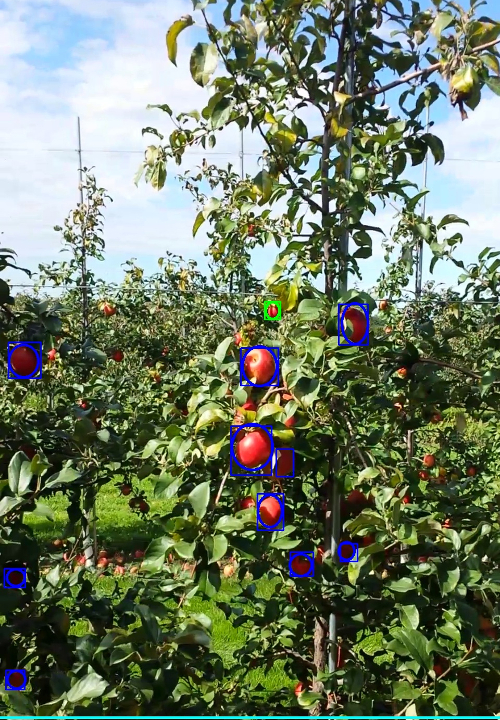
\includegraphics[width=0.3\columnwidth]{figures/prelim/tracking33.jpg}
%%%
\caption{
Tracking apples across three consecutive images. Leftmost image is the first frame. In consecutive frames, apples detected earlier are shown in blue. New apples are circled green. \label{fig:tracking}}
}
\end{figure}


\section{Merging Scene Geometry from Both Sides}\label{subsec:sysmergecount}
This component takes the single side reconstructions as input and outputs a merged reconstructions~\cite{roy_registering_2018}. Merging the two side-reconstructions is difficult due to the lack of overlap between the two partial reconstructions. We present a novel method that utilizes global features to constrain the solution. Specifically, we use information from the silhouettes and the ground plane for alignment. This component is presented in details at Chapter~\ref{chapter:merge_both}.

\section{Fruit Yield Estimation}\label{sec:fruityield}
This component takes the fruit counts from single sides, the merged reconstructions and computes the combined fruit count for the captured portion of the tree row. It takes care of eliminating fruits on the ground and on other rows, and double counting due to fruits visible from both sides. This component is described in detail at Chapter~\ref{chapter:merge_both}. Next we discuss an independent component that we developed for counting fruits in an active perception settings.

\section{Active Fruit Counting}\label{sec:activecounting}
Current systems for automated yield mapping involve the capture of imagery along an arbitrary and/or predetermined path. This approach is sufficient for large commercial orchards which have ``fruit-walls" where the fruits are visible from the outside and the clusters contain a small number of fruits. However, in more general settings, estimating the exact count from an arbitrary view is difficult. See Figure~\ref{fig:compl}. In chapter~\ref{chapter:active_counting} we show how active vision techniques can be used to accurately obtain the number of apples in a cluster. Consider a system where a robot equipped with a controllable camera is charged with surveying an orchard (Figure~\ref{fig:robotplatform}). Imagine that the robot positions the base near a tree and obtains the first view of an apple cluster. Where should it take the second image from so as to accurately estimate the number of apples in the cluster? We study this novel active perception problem in chapter~\ref{chapter:active_counting}.

With the problem formulation and different sub-problems of interest clearly stated, we are now ready to position this proposal with respect to the existing literature.
%
%In this proposal, we present an end-to-end computer vision system for yield estimation in apple orchards. Our approach can merge fruit counts from both sides of a tree row without reliance on any specialized hardware. Additionally, the system allows flexibility in exchanging individual components of the system.


\section{Contributions of the Proposal}\label{sec:intro_contrib}
Next we discuss the technical contributions of this proposal.
\subsection{Fruit Detection}rrr
Varying colors of apples (red, golden, green, yellow along with the mixture of their shades), different lighting conditions, shadows and occlusions created by leaves and branches make the job of identifying apples from images difficult. Earlier methods for fruit detection relied on color thresholds and controlled lighting. More recent techniques are dominated by deep learning techniques (See [7] Section 2 for a comprehensive review). These methods require a large amount of training data though. Generating such training data for different varieties of apples, in different lighting conditions are tedious and cumbersome.  In [7], we present a semi-supervised segmentation method which utilizes minimal user interaction to train a classification model and uses it to identify the apples. Additionally, the system can store trained models that can be used for a similar variety of apples and lighting conditions. Our method does not rely on detecting every apple in a single frame. We utilize multiple views for detection based on the assumption that for every apple there is some view from which it is detected. This provides robustness against false positives and helps us achieve high precision and recall.

\subsection{Counting Fruits from Clusters}
Counting apples from a running sequence of images is difficult as apples can be found in arbitrarily shaped clusters in which almost all apples overlap with each other. Furthermore, because of specularities as well as occlusions due to leaves and branches, some apples are not detectable at all. Existing solutions for counting fruits are dominated by circular Hough transform (CHT). The main bottleneck of using CHT is that the parameters need to be tuned across different datasets.  In [2,7], we present a method for counting based on a classic clustering technique: Gaussian Mixture Models (GMM) [8]. We model each apple with a Gaussian probability distribution function and each apple cluster with a mixture of Gaussians. We present a novel heuristic to find the correct number of components (i.e. the number of apples) in the mixture model. Additionally, we merge the information obtained from the per frame operations across multiple frames utilizing camera motion.\\

\subsection{Recovering Scene Geometry Using Fruits as Features}
To track fruits accurately, we need to recover the geometry of the underlying scene. This is one of the most fundamental problems in computer vision known as Structure from Motion (SfM). Baseline SfM methods fail to align dense apple clusters across multiple frames resulting in the same apple being registered multiple times. In [3], we proposed a novel SfM pipeline where apple contours are directly used for generating dense point matches. These matches are then used for estimating the motion of the camera and reconstructing the apples in 3D. 

\subsection{Merging Scene Geometry from Both Sides of the Tree Rows}


\subsection{Active View Planning for Counting} 
As mentioned earlier, current systems for automated yield mapping involve the capture of imagery along an arbitrary and/or predetermined path. This is sufficient for large commercial orchards where the fruits are visible from the outside and the clusters contain a small number of fruits. In more general settings though, estimating the exact count from an arbitrary view is difficult. Consider a system where a robot equipped with a controllable camera is charged with surveying an orchard. Imagine that the robot positions itself near a tree and obtains the first view of an apple cluster. Where should it take the second image from - to accurately estimate the number of apples in the cluster? In [1], we study this novel active perception problem. Our approach can be summarized as follows: Consider the set of all possible “world states” where each world state encodes the position and diameter of each apple. The images acquired by the robot associate likelihoods to these worldviews. Our goal is to plan views that reduce the entropy of this distribution sufficiently so that we can estimate the count accurately. Our main contributions in [1] are a technique to efficiently enumerate only combinatorially distinct world states, and a method to estimate their likelihoods from these images. 